\chapter{Cosmology Lecture 2: From the Expanding Metric to Friedmann's Equation}

We were talking last time about the metric of space. This lecture picks up exactly there and asks the next question: what equation tells the scale factor how to change with time? Susskind announces the plan immediately. First a little geometry, then dynamics; and the dynamics, at least for now, will be derived not from general relativity but from Newton's equations. That choice gives the lecture its shape. We begin with an expanding comoving grid, pass through a deliberately simple projectile problem, and then watch that one-body Newtonian problem turn into Friedmann's equation. The selected board frames are kept below as local mathematical evidence, following Leonard Susskind's lecture with supporting curation from LazyingArt LLC and Video2Book.

\section{From Homogeneity to the Expanding Metric}

The standing assumptions are homogeneity and isotropy. Under those assumptions Hubble's law is not something tacked on from observation after the fact; it is the natural kinematics of a uniformly expanding universe. At a fixed time,
\begin{equation}
v = H(t)\,d.
\end{equation}
The proportionality is linear in the distance, and the important qualification comes immediately: the so-called Hubble constant is constant in space, not in time. Homogeneity means it does not vary from place to place. It does \emph{not} mean it remains unchanged as the universe evolves.

Before writing any metric, Susskind pauses over the question of measuring rods. If space expands, why do meter sticks not expand? The lecture's answer is concrete. The forces binding ordinary matter are enormously stronger than the tiny effect of cosmological expansion on atomic scales. One may imagine adding a minuscule extra repulsion between atoms; it would shift an equilibrium separation a little, but it would not tear apart a tightly bound rod. The cosmological expansion is therefore seen not in bound objects but in the growing separation of sufficiently distant, sufficiently unbound systems such as galaxies.

This is the reason for comoving coordinates. We assign coordinates that move with the Hubble flow. A galaxy with no extra peculiar motion then keeps the same coordinate value for all time. What changes is the relation between coordinate separation and physical distance measured in meters. That changing conversion factor is the scale factor \(a(t)\).

For flat space the spatial line element is
\begin{equation}
ds^2 = a(t)^2\left(dx^2+dy^2+dz^2\right).
\end{equation}
Here \(x,y,z\) are comoving coordinates. If two galaxies have a fixed coordinate separation \(\Delta x\) along one axis, then their physical distance is
\begin{equation}
d(t)=a(t)\,\Delta x.
\end{equation}
Differentiating with respect to time gives
\begin{equation}
v=\dot d=\dot a\,\Delta x=\frac{\dot a}{a}\,d.
\end{equation}
So once the comoving metric is in hand, the Hubble parameter becomes
\begin{equation}
H(t)=\frac{\dot a}{a}.
\end{equation}
That is already the first bridge from geometry to dynamics.

\section{Flat Spatial Slices Inside Curved Spacetime}

Now we shift from the metric of space to the metric of spacetime. The lecture insists on an important point: three-dimensional space may be flat while spacetime is nevertheless curved. If the geometry of space changes with time, then spacetime is no longer Minkowski even if each spatial slice remains flat. Susskind's image is a flat rubber sheet being stretched by distant giants. The sheet stays flat as a sheet, but the four-dimensional history is curved.

Starting from the special-relativistic form \(d\tau^2=dt^2-ds^2\), we upgrade the spatial metric to
\begin{equation}
d\tau^2 = dt^2 - a(t)^2\left(dx^2+dy^2+dz^2\right).
\end{equation}
The coefficients do not depend on position in space; they depend only on time. That is the metric expression of homogeneity. In matrix language, completing the spoken board description in the standard way, one writes
\begin{equation}
g_{\mu\nu}=\mathrm{diag}\!\left(1,-a(t)^2,-a(t)^2,-a(t)^2\right).
\end{equation}
The off-diagonal terms vanish. There are no \(dx\,dy\) or \(dx\,dt\) terms. The metric is almost as simple as that of flat spacetime, except that the conversion between spatial separation and time is now time-dependent.

\begin{figure}
\centering

\includegraphics[width=0.58\textwidth]{lecture_02_figure_02.png}

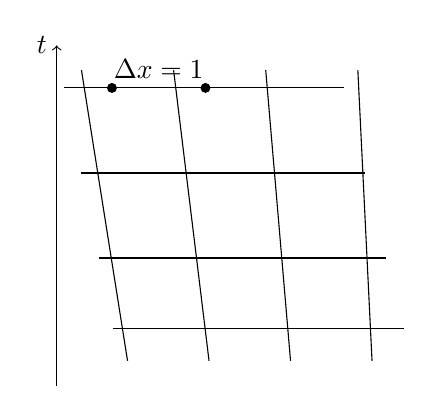
\begin{tikzpicture}[scale=0.9]
\draw[->] (0,0) -- (0,4.8) node[left]{\(t\)};
\draw (0.8,0.8) -- (4.9,0.8);
\draw (0.6,1.8) -- (4.65,1.8);
\draw (0.35,3.0) -- (4.35,3.0);
\draw (0.1,4.2) -- (4.05,4.2);

\draw (1.0,0.35) -- (0.35,4.45);
\draw (2.15,0.35) -- (1.65,4.45);
\draw (3.3,0.35) -- (2.95,4.45);
\draw (4.45,0.35) -- (4.25,4.45);

\fill (0.78,4.2) circle (2pt);
\fill (2.10,4.2) circle (2pt);
\node[above] at (1.44,4.2) {\(\Delta x=1\)};
\end{tikzpicture}
\caption{Spacetime interval and expanding-grid sketch. The lecture frame is retained as board evidence; the redraw beneath it makes the comoving grid legible as a geometric cartoon of fixed coordinate separation and increasing physical distance.}
\end{figure}

The picture is not decoration. It carries the lecture's intuition. Alice and Bob remain one coordinate unit apart, but one coordinate unit comes to represent more and more physical distance as time goes on. If \(a(t)\) were driven to zero, then every physical separation would be driven to zero with it. In the lecture this is said in plain language: everything gets squashed on top of everything else, and the density becomes infinite. If \(a(t)\) grows, the universe becomes correspondingly more diffuse.

There is another subtle point here. This metric has the stated form only in the frame moving with the galaxies. Rotations leave the spatial part unchanged, but a Lorentz boost does not preserve the same isotropic appearance. Matter itself picks out the preferred comoving frame.

\subsection{Question \& Answer}

\paragraph{Whose time is \(t\) in \(a(t)\)?}
It is the time measured by clocks moving with the galaxies. The lecture even says: imagine a cosmic clock factory making identical clocks, one carried by each galaxy. The coordinate time \(t\) is the time those comoving clocks measure.

This is also immediate from the metric. Along a galaxy worldline in the comoving frame we have
\begin{equation}
dx=dy=dz=0,
\end{equation}
so the interval reduces to
\begin{equation}
d\tau^2=dt^2,
\end{equation}
hence
\begin{equation}
dt=d\tau.
\end{equation}
So the time appearing in \(a(t)\) is cosmic proper time along the flow lines of the galaxies.

\section{Newtonian Warm-Up: A Projectile in a Gravitational Field}

With the geometry fixed, Susskind makes the lecture's second major pivot. Rather than deriving the dynamics of \(a(t)\) from general relativity, he cools the problem down first and goes back to a familiar Newtonian one-body system. Before doing cosmology, let us understand a particle ejected radially outward from a heavy gravitating mass.

Take a heavy mass \(M\) and a much smaller mass \(m\). Give the small mass an outward impulse and then let it move freely under gravity. Angular complications are not the point here, so the motion is taken to be radial. What matters for the cosmological analogy is energy conservation.

The kinetic energy is
\begin{equation}
\frac{1}{2}mv^2.
\end{equation}
The gravitational potential energy has the product of the masses, Newton's constant, and one power of the distance in the denominator:
\begin{equation}
-\frac{GMm}{d}.
\end{equation}
On the board the factors are written in the order \(mMG/D\); in the cleaned equations we restore the conventional form \(GMm/d\), but the board order is kept visible in the screenshots below. The conserved total energy is then
\begin{equation}
E=\frac{1}{2}mv^2-\frac{GMm}{d}.
\end{equation}
Here ``constant'' means constant in time for the particular particle under discussion. Different projectiles may of course have different values of \(E\).

\begin{figure}
\centering

\includegraphics[width=0.44\textwidth]{lecture_02_figure_03.png}
\hfill

\includegraphics[width=0.44\textwidth]{lecture_02_figure_04.png}

\begin{tikzpicture}[scale=1.0]
\draw (0,0) circle (0.42);
\draw (0,0) circle (0.28);
\draw (0,0) circle (0.14);
\node at (0,-0.8) {\(M\)};

\fill (1.25,0) circle (2pt);
\node[below] at (1.25,0) {\(m\)};
\draw[->] (1.35,0) -- (3.0,0);

\node at (5.0,0.4) {\(\frac{1}{2}mv^2\)};
\node at (7.4,0.4) {\(-\)};
\node at (9.1,0.4) {\(\frac{GMm}{d}\)};
\end{tikzpicture}
\caption{The Newtonian warm-up in the same order as the board. First the kinetic term, then the full energy balance with negative gravitational potential. The redraw regularizes the source--test-mass geometry without replacing the lecture frames.}
\end{figure}

Notice how the lecture builds the formula. First the kinetic term is written. Then the potential term is added. Only after that does the negative sign become the issue. The sequence matters because later the cosmological argument will lean on the same intuition: not just on the existence of a formula, but on what the sign of the gravitational term means.

\subsection{Question \& Answer}

\paragraph{Why is the gravitational potential energy negative?}
The lecture does not answer this by abstract convention. It answers it by drawing the graphs of \(1/D\) and \(-1/D\). Forget the constants. The function \(1/D\) decreases as \(D\) increases. The function \(-1/D\) is the same curve upside down. Forces push in the direction of decreasing potential energy. Therefore an attractive force, which pulls inward toward smaller \(D\), must correspond to the upside-down curve:
\begin{equation}
V(d)\propto -\frac{1}{d}.
\end{equation}
Bringing the mass closer to the source creates a larger amount of negative potential energy. Moving it farther away makes the energy less negative. That is exactly what attraction means in energy language.

\begin{figure}
\centering

\includegraphics[width=0.46\textwidth]{lecture_02_figure_05.png}

\begin{tikzpicture}[scale=1.0]
\draw[->] (0,0) -- (4.6,0) node[right]{\(D\)};
\draw[->] (0,-2.2) -- (0,2.2);

\draw[domain=0.35:4.0,smooth,variable=\x] plot (\x,{1/\x});
\draw[domain=0.35:4.0,smooth,variable=\x] plot (\x,{-1/\x});

\node at (3.35,0.95) {\(\frac{1}{D}\)};
\node at (3.35,-1.0) {\(-\frac{1}{D}\)};
\end{tikzpicture}
\caption{Qualitative potential-energy graphs. The lecture frame is kept because it records the actual board argument; the redraw regularizes the axes and the two comparison curves \(1/D\) and \(-1/D\).}
\end{figure}

\section{Escape Velocity and the Three Energy Regimes}

Once the conserved energy is on the board, the lecture does not calculate right away. Instead it classifies the possible motions. There are only three cases.

\begin{itemize}
\item If \(E<0\), the motion is bound. The particle rises, slows, turns around, and falls back.
\item If \(E=0\), the particle has exactly the escape velocity. The distance keeps increasing forever, while the speed decreases toward zero.
\item If \(E>0\), the particle escapes completely. Gravity still decelerates it for a while, but not enough to prevent a nonzero asymptotic outward speed.
\end{itemize}

The critical case \(E=0\) needs to be heard carefully. The distance is unbounded, but the speed goes to zero. It cannot actually come to rest at any finite time, because if it did, it would turn around and fall back. So the speed decreases forever without ever quite reaching zero at finite time.

For sufficiently small starting velocity the potential term dominates from the beginning, so the energy is negative:
\begin{figure}
\centering

\includegraphics[width=0.62\textwidth]{lecture_02_figure_06.png}
\caption{Later emphasis frame: at small enough initial outward speed, the negative potential term dominates the total energy.}
\end{figure}

This is the bridge to cosmology. The universe, in Newtonian language, behaves the same way. If the initial Hubble flow is large enough, galaxies escape from one another forever. If it is too small, gravity eventually wins and the universe recollapses. Between the two lies the critical case, the cosmological analog of escape velocity.

\section{Newton's Shell Theorem and the Cosmological Reduction}

The projectile analogy becomes a cosmological calculation only because of Newton's shell theorem. This is the lecture's third hinge, and Susskind takes time to make the audience trust it.

For a spherically symmetric mass distribution, the gravitational force on a particle at radius \(d\) is exactly the same as if all the mass inside radius \(d\) were concentrated at the center, while the mass outside radius \(d\) contributes no net force. The theorem is stronger than the familiar outside-a-sphere statement. A perfect spherical shell exerts no force on a particle anywhere inside it, even off-center. This is a surprising property, and in the lecture Susskind reminds us that it is special to the inverse-square law.

He even sketches a water-flow analogy: a point source produces a \(1/r^2\)-type flux in three dimensions, and a symmetric shell of such sources produces no net interior flow. The details are postponed, but the moral is clear. Exterior shells cancel.

Now we use that theorem in cosmology. Pick any galaxy and, for the sake of calculation, call it the center. Because the universe is homogeneous and isotropic, this choice cannot matter. Pick a second galaxy at comoving coordinate \(x\). Draw a sphere centered on the first galaxy and passing through the second. Then only the mass inside that sphere matters for the motion of the second galaxy.

Two further facts are essential.

First, the center is arbitrary. We could have centered the calculation on Alice, Bob, Fred, or any other galaxy, and the same equation must come out.

Second, the sphere expands with the Hubble flow. It therefore encloses the same galaxies for all time, and so its enclosed mass is constant in time even though its physical radius changes.

\section{From Galaxy Energetics to Friedmann's Equation}

We are now ready to write for a galaxy exactly the same kind of Newtonian energy equation we wrote for the projectile. After dividing by the test mass, it is convenient to write
\begin{equation}
\frac{v^2}{2}-\frac{GM(d)}{d}=\varepsilon(x),
\end{equation}
where \(\varepsilon(x)\) is constant in time for the galaxy at comoving coordinate \(x\). It is not required to be the same for every \(x\).

The physical distance from the chosen center to that galaxy is
\begin{equation}
d=a(t)x,
\end{equation}
and because \(x\) is comoving,
\begin{equation}
v=\dot d=\dot a\,x.
\end{equation}
If \(\rho(t)\) is the homogeneous density, then the enclosed mass is
\begin{equation}
M(d)=\frac{4\pi}{3}\rho\,d^3=\frac{4\pi}{3}\rho\,a^3x^3.
\end{equation}
Substituting these into the energy equation gives
\begin{align}
\frac{(\dot a x)^2}{2}-\frac{G\left(\frac{4\pi}{3}\rho\,a^3x^3\right)}{ax} &= \varepsilon(x), \\
\frac{\dot a^2x^2}{2}-\frac{4\pi G}{3}\rho\,a^2x^2 &= \varepsilon(x).
\end{align}

Here the lecture lingers on the factor of \(x^2\), and rightly so. Both terms on the left-hand side are proportional to \(x^2\). Everything else there is the same for every galaxy. Therefore the right-hand side must also be proportional to \(x^2\). That is the precise meaning of the seemingly casual statement that the ``constant'' must scale with \(x^2\). The farther galaxies carry larger energies, and that is exactly what one should expect since they are also moving faster.

So we write
\begin{equation}
\varepsilon(x)=-\frac{k}{2}\,x^2,
\end{equation}
where the normalization of \(k\) is conventional. Dividing through by \(x^2/2\), we obtain
\begin{equation}
\dot a^2=\frac{8\pi G}{3}\rho\,a^2-k.
\end{equation}
Dividing once more by \(a^2\), we arrive at the standard historical form,
\begin{equation}
\left(\frac{\dot a}{a}\right)^2=\frac{8\pi G}{3}\rho-\frac{k}{a^2}.
\end{equation}

This is Friedmann's equation in the Newtonian form emphasized in the lecture. One can also write it as
\begin{equation}
H(t)^2=\frac{8\pi G}{3}\rho-\frac{k}{a^2},
\end{equation}
since \(H=\dot a/a\). Susskind likes to pause here and point out the historical drama of the result: a purely Newtonian energy argument has landed on the same equation that later appears as a component of Einstein's equations.

The sign of \(k\) tracks the same three cases we already met in the escape-velocity problem. The critical case is \(k=0\). In units with \(c=1\), \(k\) is dimensionless.

\section{Matter Density, the Critical Case, and the Age of the Universe}

If we sent ourselves home at this point and tried to solve Friedmann's equation, the first objection would be immediate: \(\rho\) is not a constant. It changes as the universe expands. So the next task is to express that dependence cleanly.

Susskind does it with a unit comoving cube. Take a cube that is one unit on a side in coordinate space. The galaxies move with the comoving coordinates, so the same galaxies remain inside that cube for all time. Let the mass inside it be \(m_{\Box}\). Then the physical side length of the cube is \(a(t)\), and the physical volume is \(a(t)^3\). Therefore
\begin{equation}
\rho(t)=\frac{m_{\Box}}{a(t)^3}.
\end{equation}

Substituting this into Friedmann's equation gives
\begin{equation}
\left(\frac{\dot a}{a}\right)^2=\frac{8\pi G\,m_{\Box}}{3a^3}-\frac{k}{a^2}.
\end{equation}
Now choose the simplest case, \(k=0\), the analog of exact escape velocity. Then
\begin{equation}
\left(\frac{\dot a}{a}\right)^2=\frac{8\pi G\,m_{\Box}}{3a^3}.
\end{equation}

Before solving, the lecture points out a qualitative consequence. The right-hand side is always positive. Therefore the left-hand side cannot pass through zero, which means the model does not turn around. In the critical case the universe expands forever, but with a continually decreasing expansion rate.

Now comes the worked solution. Rather than grinding through the differential equation abstractly, Susskind tries a power law:
\begin{equation}
a(t)=ct^p.
\end{equation}
Then
\begin{align}
\dot a &= cp\,t^{p-1}, &
\frac{\dot a}{a} &= \frac{p}{t}.
\end{align}
Substituting into the equation gives
\begin{equation}
\frac{p^2}{t^2}=\frac{8\pi G\,m_{\Box}}{3c^3\,t^{3p}}.
\end{equation}
For this to hold for all \(t\), the powers of \(t\) must match:
\begin{equation}
3p=2.
\end{equation}
So
\begin{equation}
p=\frac{2}{3}.
\end{equation}
Then matching coefficients gives
\begin{equation}
\frac{4}{9}=\frac{8\pi G\,m_{\Box}}{3c^3},
\end{equation}
hence
\begin{equation}
c^3=6\pi G\,m_{\Box}.
\end{equation}
The critical matter-dominated solution is therefore
\begin{equation}
a(t)=\left(6\pi G\,m_{\Box}\right)^{1/3}t^{2/3}.
\end{equation}
More generally one may absorb the remaining integration constant into a shift of the origin of time and write
\begin{equation}
a(t)\propto (t-t_0)^{2/3}.
\end{equation}

This is a more interesting result than it may look at first sight. The universe does not expand linearly with time. Linear growth would be the analog of unaccelerated motion. Here the growth is slower than linear:
\begin{equation}
a(t)\propto t^{2/3}.
\end{equation}
So the expansion slows down, but in the critical case it never turns around.

The interpretation of \(t=0\) is also part of the lecture's rhythm. If \(a(t)\) really went to zero, everything would be squashed on top of everything else and the density would diverge. Susskind immediately softens the literalness of that statement: the Newtonian model cannot be trusted all the way down to infinite density. But it does tell us that the universe emerged from an extremely dense early state. That is the Big Bang limit of the model.

The Hubble parameter now becomes explicit:
\begin{equation}
H(t)=\frac{\dot a}{a}=\frac{2}{3t}.
\end{equation}
So in this model
\begin{equation}
t=\frac{2}{3H}.
\end{equation}
This is one of the lecture's payoffs. The Hubble constant is not a constant at all; it falls like \(1/t\). Susskind jokes that a final examination could consist of a single question: \emph{Is the Hubble constant a constant?} The correct answer is no.

The same formula turns a present-day measurement of \(H\) into an age estimate. In the lecture Susskind quotes an age of roughly \(13\) to \(14\) billion years and remarks that \(k=0\) is observationally very realistic, with no known significant deviation from flatness at the level of precision he quotes.

\subsection{Question \& Answer}

\paragraph{Why does the age estimate not depend on the arbitrary fiducial box mass?}
The lecture's late discussion of this point is subtle because the notation becomes slippery, but the underlying idea is clean. The fiducial comoving box is conventional. If we double its side length, then the mass inside it grows by a factor of \(8\), while \(m_{\Box}^{1/3}\) grows by a factor of \(2\). The corresponding normalization of \(a\) changes by the same factor. What is physical is the density
\begin{equation}
\rho=\frac{m_{\Box}}{a^3},
\end{equation}
or equivalently the invariant combination \(a/m_{\Box}^{1/3}\), not \(a\) and \(m_{\Box}\) taken separately.

The cancellation appears directly in the solution. If
\begin{equation}
a(t)=ct^{2/3},
\end{equation}
then
\begin{equation}
\dot a=\frac{2}{3}c\,t^{-1/3},
\end{equation}
so
\begin{equation}
\frac{\dot a}{a}=\frac{\frac{2}{3}c\,t^{-1/3}}{ct^{2/3}}=\frac{2}{3t}.
\end{equation}
The constant \(c\), and therefore the dependence on the fiducial-box mass, drops out of \(H=\dot a/a\). That is why the age relation
\begin{equation}
t=\frac{2}{3H}
\end{equation}
does not depend on the arbitrary normalization of the comoving box in the critical model.

This is also the right place to hear the lecture's last reinterpretation. Rearranging Friedmann's equation gives
\begin{equation}
\frac{\dot a^2}{a^2}-\frac{k}{a^2}=\frac{8\pi G}{3}\rho.
\end{equation}
The left-hand side is geometric: it is built from the scale factor and, next time, from spatial curvature. The right-hand side is matter density, or in relativistic language energy density. That is exactly the sort of equation Einstein's theory ought to produce.

\section{Summary}

The lecture unfolds in a very deliberate sequence. Homogeneity and isotropy fix the kinematics of expansion. The comoving metric gives the scale factor a precise meaning. A Newtonian projectile problem provides the right intuition for conserved energy and escape velocity. Newton's shell theorem then converts the many-body universe into an effective one-body problem, and that reduction yields
\begin{equation}
\left(\frac{\dot a}{a}\right)^2=\frac{8\pi G}{3}\rho-\frac{k}{a^2}.
\end{equation}
In the critical matter-dominated case \(k=0\), the solution is
\begin{equation}
a(t)\propto t^{2/3}, \qquad H(t)=\frac{2}{3t}.
\end{equation}
So the Newtonian model already gives a serious cosmological prediction: a slowing but never reversing critical expansion, together with an age estimate from the present Hubble parameter. The next lecture will reopen the equation from the relativistic side and show how curvature and Einstein's equations complete the story.